\documentclass[12pt]{report}
\usepackage[utf8]{inputenc}
\usepackage[russian]{babel}
%\usepackage[14pt]{extsizes}
\usepackage{listings}
\usepackage{graphicx}
\usepackage{amsmath,amsfonts,amssymb,amsthm,mathtools} 
\usepackage{pdfpages}

% Для листинга кода:
\lstset{ %
language=python,               
basicstyle=\small\sffamily, % размер и начертание шрифта для подсветки кода
numbers=left,               % где поставить нумерацию строк (слева\справа)
numberstyle=\tiny,           % размер шрифта для номеров строк
stepnumber=1,                   % размер шага между двумя номерами строк
numbersep=5pt,                % как далеко отстоят номера строк от подсвечиваемого кода
showspaces=false,            % показывать или нет пробелы специальными отступами
showstringspaces=false,      % показывать или нет пробелы в строках
showtabs=false,             % показывать или нет табуляцию в строках
frame=single,              % рисовать рамку вокруг кода
tabsize=2,                 % размер табуляции по умолчанию равен 2 пробелам
captionpos=t,              % позиция заголовка вверху [t] или внизу [b] 
breaklines=true,           % автоматически переносить строки (да\нет)
breakatwhitespace=false, % переносить строки только если есть пробел
escapeinside={\#*}{*)}   % если нужно добавить комментарии в коде
}

% Для измененных титулов глав:
\usepackage{titlesec, blindtext, color} % подключаем нужные пакеты
\definecolor{gray75}{gray}{0.75} % определяем цвет
\newcommand{\hsp}{\hspace{20pt}} % длина линии в 20pt
% titleformat определяет стиль
\titleformat{\chapter}[hang]{\Huge\bfseries}{\thechapter\hsp\textcolor{gray75}{|}\hsp}{0pt}{\Huge\bfseries}


% plot
\usepackage{pgfplots}
\usepackage{filecontents}
\usetikzlibrary{datavisualization}
\usetikzlibrary{datavisualization.formats.functions}
\begin{filecontents}{StandartGood.dat}
100 277106300
200 2223427800
300 7539788600
400 17871861900
500 40937160400
\end{filecontents}

\begin{filecontents}{WinogradGood.dat}
100 316336900
200 2625659200
300 8886568400
400 21390493800
500 47627553100
\end{filecontents}

\begin{filecontents}{WinogradImpGood.dat}
100 294409400
200 2411611600
300 8231789400
400 20014957200
500 44288032900
\end{filecontents}

\begin{filecontents}{StandartBad.dat}
101 270037100
201 2264925400
301 7560858300
401 17928154700
501 38945951700
\end{filecontents}

\begin{filecontents}{WinogradBad.dat}
101 320120100
201 2673975500
301 8936763900
401 21574541600
501 47350318700
\end{filecontents}

\begin{filecontents}{WinogradImpBad.dat}
101 297891600
201 2491565200
301 8241902300
401 20112025300
501 44380396700
\end{filecontents}


\begin{document}
%\def\chaptername{} % убирает "Глава"

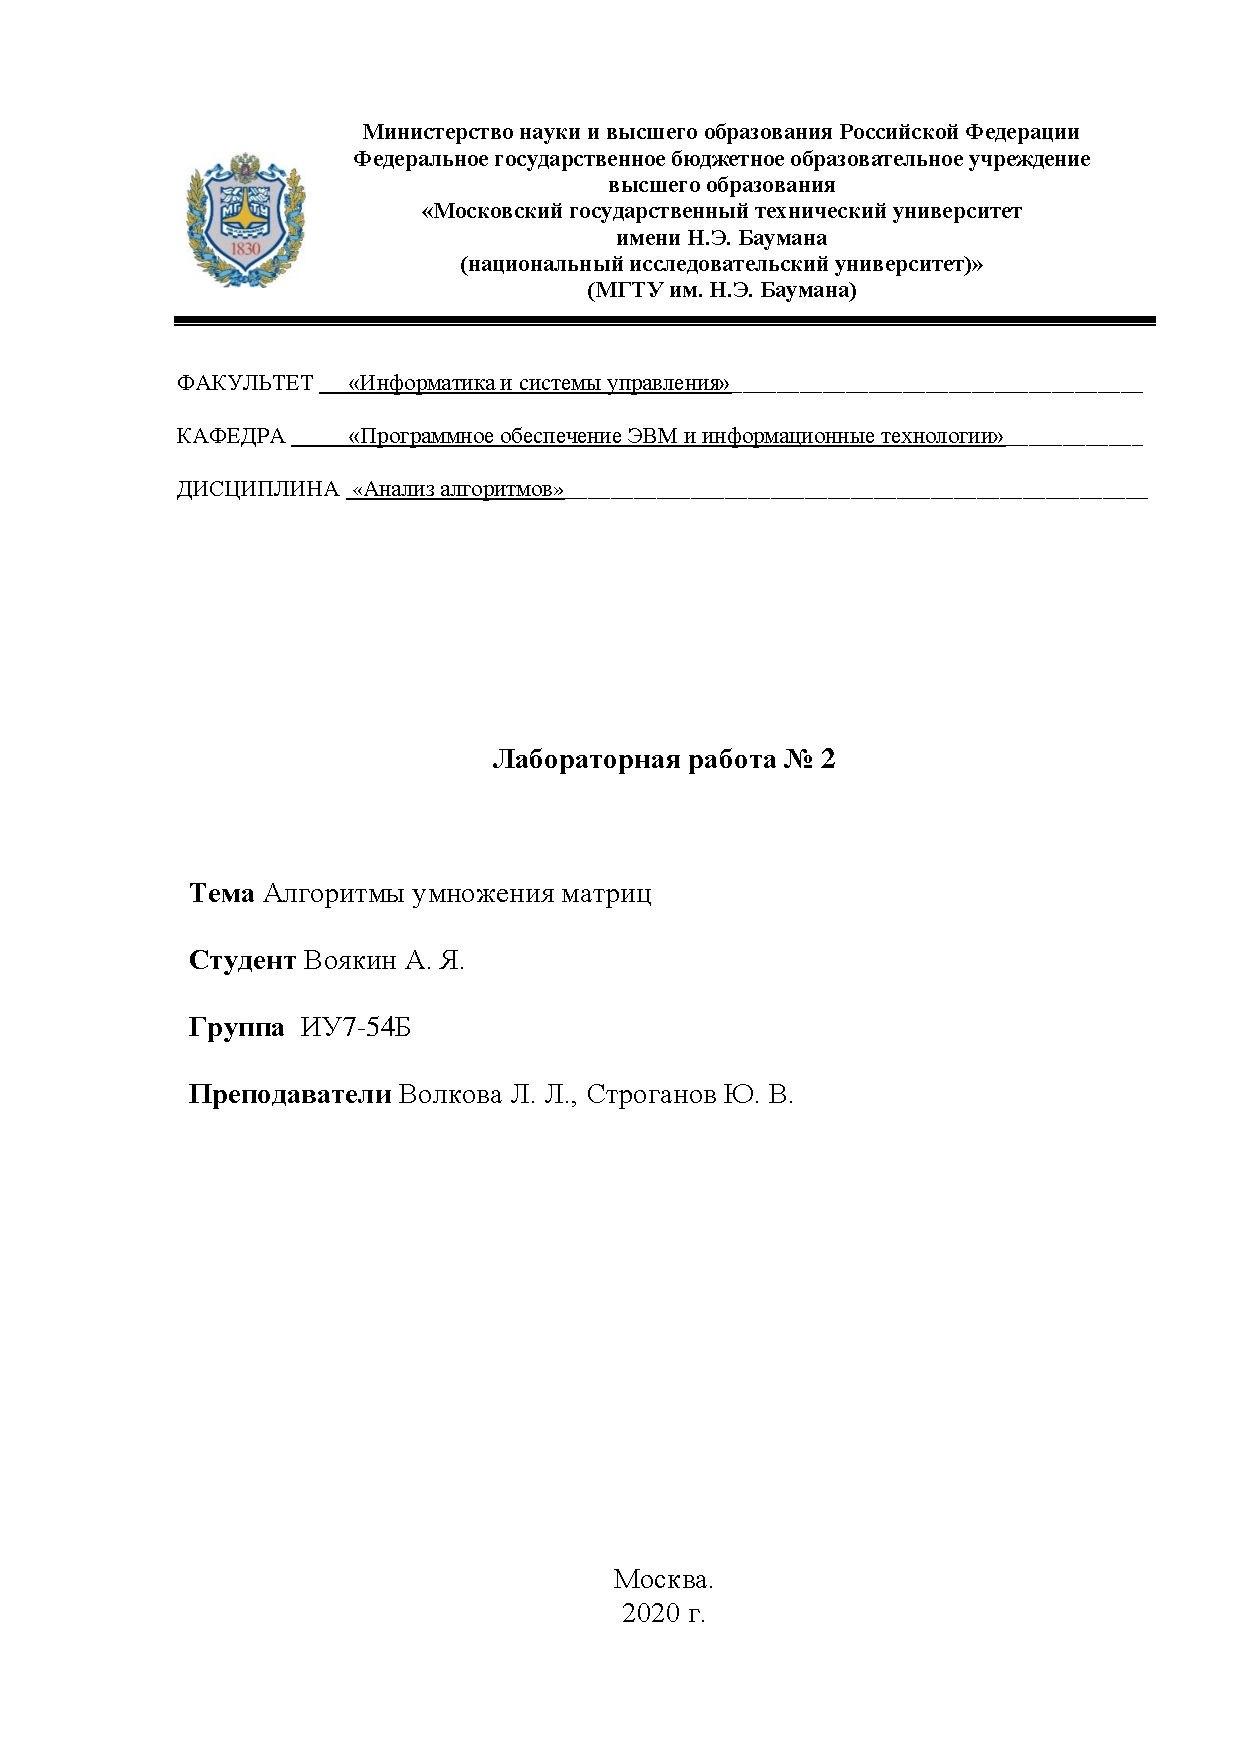
\includepdf{Title.pdf}

\tableofcontents

\newpage
\chapter*{Введение}
\addcontentsline{toc}{chapter}{Введение}
Цель работы - изучение алгоритмов умножения матриц. В данной лабораторной работе рассматривается стандартный алгоритм умножения матриц, алгоритм Винограда и модифицированный алгоритм Винограда. Также требуется провести рассчет сложности алгоритмов, получить навыки в оптимизации алгоритмов.
Использованные алгоритмы активно применяются во всех областях, применяющих линейную алгебру, таких как:
\begin{itemize}
	\item компьютерная графика;
	\item физика;
	\item экономика;
	\item прочее.
\end{itemize}

В ходе лабораторной работы предстоит:
\begin{itemize}
	\item изучить алгоритмы умножения матриц: стандартный и алгоритм Винограда;
	\item улучшить алгоритм Винограда;
	\item дать теоретическую оценку базового алгоритма умножения матриц, алгоритма Винограда и улучшенного алгоритма Винограда;
	\item реализовать три алгоритма умножения матриц на одном из языков программирования;
	\item сравнить алгоритмы умножения матриц.
\end{itemize}





\chapter{Аналитическая часть}
Матрица - математический объект, эквивалентный двумерному массиву. Числа располагаются в матрице по строкам и столбцам. Если число столбцов в первой матрице совпадает с числом строк во второй, то эти две матрицы можно перемножить. У произведения будет столько же строк, сколько в первой матрице, и столько же столбцов, сколько во второй. Постановка задачи перемножения матриц описана в [1].
	    
\section{Классический алгоритм умножения матриц}
Пусть даны две прямоугольные матрицы А и В размерности m на n и n на l соответсвенно: 
\[ \begin{bmatrix}
a_{1,1} & ... & a_{1,n} \\
... & ... & ... \\
a_{m,1} & ... & a_{m,n} \\
\end{bmatrix} \]\\

\[ \begin{bmatrix}
b_{1,1} & ... & b_{1,l} \\
... & ... & ... \\
b_{n,1} & ... & b_{n,l} \\
\end{bmatrix} \]\\

В результате получим матрицу C размерности m на l:
	
\[ \begin{bmatrix}
c_{1,1} & ... & c_{1,l} \\
... & ... & ... \\
c_{m,1} & ... & c_{m,l} \\
\end{bmatrix} \]\\


$c_{i,j} = \sum\limits_{r=1}^n a_{i,r}\cdot b_{r,j}$ называется произведением матриц A и B.


\section{Алгоритм Винограда}

Рассмотрим два вектора $V = (v1, v2, v3, v4)$ и $W = (w1, w2, w3, w4)$.  

Их скалярное произведение равно (\ref{formula}) 

\begin{equation} \label{formula}
	V \cdot W=v_1 \cdot w_1 + v_2 \cdot w_2 + v_3 \cdot w_3 + v_4 \cdot w_4
\end{equation}

Равенство (\ref{formula}) можно переписать в виде (\ref{formula2}) 
\begin{equation} \label{formula2}
	V \cdot W=(v_1 + w_2) \cdot (v_2 + w_1) + (v_3 + w_4) \cdot (v_4 + w_3) - v_1 \cdot v_2 - v_3 \cdot v_4 - w_1 \cdot w_2 - w_3 \cdot w_4
\end{equation}

Менее очевидно, что выражение в правой части последнего равенства допускает предварительную обработку: его части можно вычислить заранее и запомнить для каждой строки первой матрицы и для каждого столбца второй. 

Это означает, что над предварительно обработанными элементами нам придется выполнять лишь первые два умножения и последующие пять сложений, а также дополнительно два сложения. Подробое описание алгоритма Винограда можно найти в [2].

В случае умножения матриц, строка и столбец которых представляют собой вектора нечётного размера, схема рассчёта элементов результирующей матрицы сохраняется. После чего, к каждому элементу $c_{i,j}$ результирующей матрицы прибавляется число $v_{i, m} \cdot u_{m, j}$, где $v_{i, m}$ - последний элемент i-той строки первой матрицы, $u_{m, j}$ - последний элемент j-того столбца второй матрицы.

\section{Вывод}
Были рассмотрены алгоритмы классического умножения матриц и алгоритм Винограда, основная отличительная черта которого — наличие предварительной обработки, а также уменьшение количества операций умножения.


\chapter{Конструкторская часть}
\section{Техническое задание}
\textbf{Требования к вводу:}\\
\begin{itemize}
	\item На вход подаются размерности матриц и сами матрицы.
\end{itemize}

\textbf{Требования к выводу:}\\
\begin{itemize}
	\item Корректное произведение введённых матриц или сообщение об ошибке в случае неккоректного ввода.
\end{itemize}


\section{Схемы алгоритмов}
В данной части будут рассмотрены схемы алгоритмов. Схема классического алгоритма умножения матриц показана на рисунке 2.1, схема алгоритма Винограда - на рисунке 2.2, схема оптимизированного алгоритма Винограда - на рисунке 2.3.

\begin{figure}[pt]
\centering
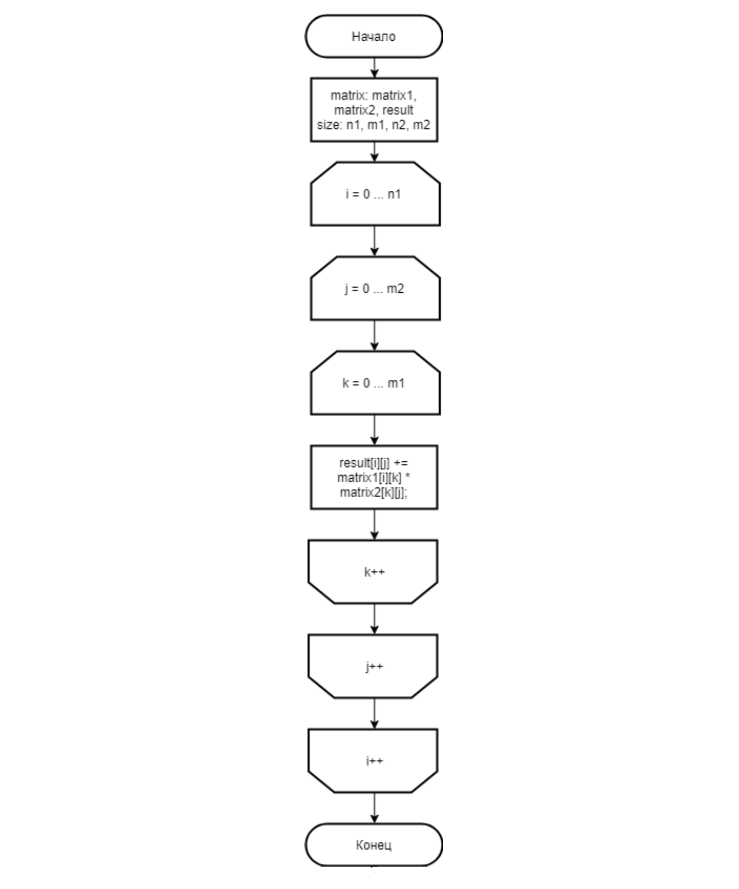
\includegraphics[scale=1]{alg1.png}
\caption{Схема классического алгоритма умножения матриц}
\label{fig:mpr}
\end{figure}

\begin{figure}[pt]
\centering
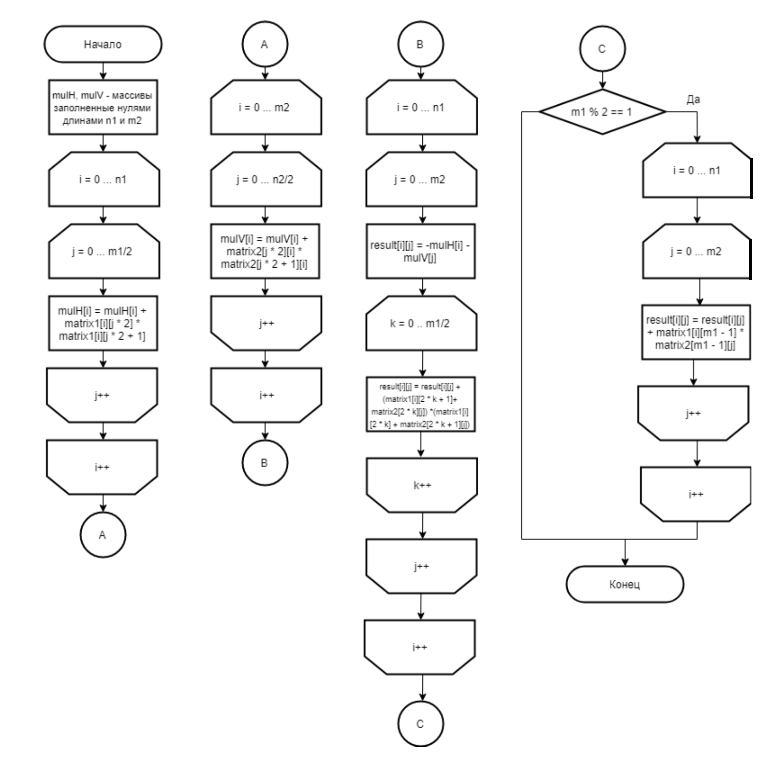
\includegraphics[scale=1]{alg2.png}
\caption{Схема алгоритма Винограда}
\label{fig:mpr}
\end{figure}


\begin{figure}[pt]
\centering
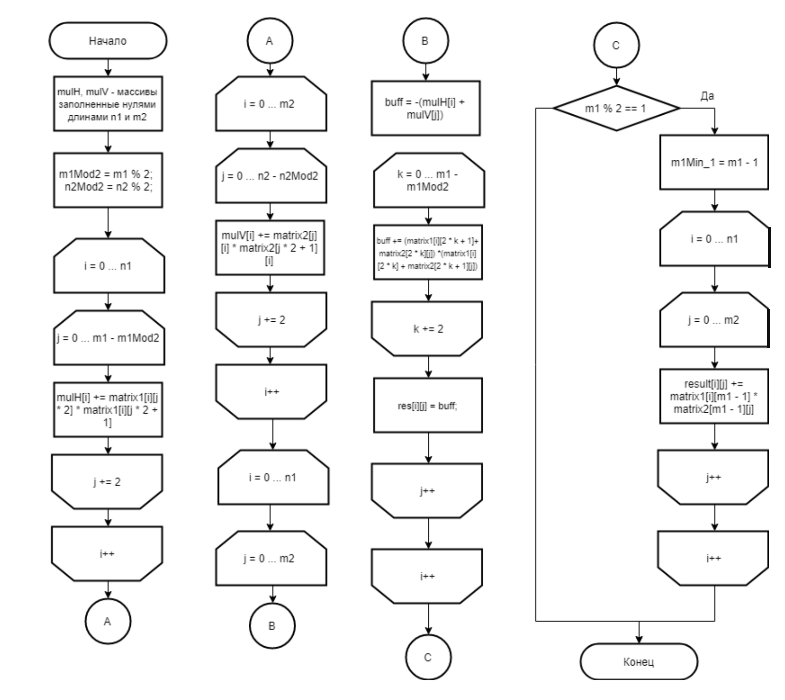
\includegraphics[scale=1]{alg3.png}
\caption{Схема оптимизированного алгоритма Винограда}
\label{fig:mpr}
\end{figure}

\newpage
\section{Трудоемкость алгоритмов}
Введем модель трудоемкости для оценки алгоритмов: 
\begin{itemize}
	\item базовые операции стоимостью 1 — +, -, *, /, =, ==, <=, >=, !=, +=, [];
	\item оценка трудоемкости цикла for от 0 до N с шагом 1 $F_{for} = 2 + N \cdot (2 + F_{body})$, где $F_{body}$ - тело цикла;
	\item стоимость условного перехода применим за 0, стоимость вычисления условия остаётся.
\end{itemize}

Оценим трудоемкость алгоритмов по коду программы.

\subsection{Классический алгоритм}
Рассмотрим трудоемкость классического алгоритма:\\

$10MNQ + 4MQ + 4 M + 2$ \\


\subsection{Алгоритм Винограда}

Рассмотрим трудоемкость алгоритма Винограда:\\

Трудоемкость алгоритма Винограда:\\

Первый цикл: $15/2 \cdot M  N + 5 \cdot M + 2$ \\

Второй цикл: $15/2 \cdot M  N + 5 \cdot M + 2$\\

Третий цикл: $13 \cdot M  N Q + 12 \cdot M Q + 4 \cdot M + 2$\\

Условный переход: $\begin{bmatrix}
             2    &&, \text{в случае невыполнения условия}\\
             15 \cdot QM + 4 \cdot M + 2 &&, \text{в случае выполнения условия}\\
           \end{bmatrix} $ \\

Итого: $15/2 \cdot M  N + 5 \cdot M + 2 + 15/2 \cdot M  N + 5 \cdot M + 2 + 13 \cdot M  N Q + 12 \cdot M Q + 4 \cdot M + 2 +
       \begin{bmatrix}
             2    &&, \text{в случае невыполнения условия}\\
             15 \cdot QM + 4 \cdot M + 2 &&, \text{в случае выполнения условия}\\
           \end{bmatrix} $ \\

\subsection{Оптимизированный алгоритм Винограда}

Рассмотрим трудоемкость алгоритма Винограда:\\

Трудоемкость алгоритма Винограда:\\

Первый цикл: $11/2 \cdot M  N + 4 \cdot M + 2$ \\

Второй цикл: $11/2 \cdot M  N + 4 \cdot M + 2$\\

Третий цикл: $17/2 \cdot M  N Q + 9 \cdot M Q + 4 \cdot M + 2$\\

Условный переход: $\begin{bmatrix}
             1    &&, \text{в случае невыполнения условия}\\
             10 \cdot QM + 4 \cdot M + 2 &&, \text{в случае выполнения условия}\\
           \end{bmatrix} $ \\

Итого: $11/2 \cdot M  N + 4 \cdot M + 2 + 11/2 \cdot M  N + 4 \cdot M + 2 + 15/2 \cdot M  N Q + 9 \cdot M Q + 4 \cdot M + 2 +
       \begin{bmatrix}
             1    &&, \text{в случае невыполнения условия}\\
             10 \cdot QM + 4 \cdot M + 2 &&, \text{в случае выполнения условия}\\
           \end{bmatrix} $ \\

\section{Вывод}
В данном разделе были рассмотрены схемы алгоритмов умножения матриц, введена модель оценки
трудоёмкости алгоритма, были рассчитаны трудоёмкости реализованных алгоримов в соответсвии 
с этой моделью.

\chapter{Технологическая часть}
\section{Выбор ЯП}
Для реализации программ был выбран язык программирования Python, ввиду наличия опыта разработки на нём. Среда разработки - PyCharm. \\

Для замера процессорного времени используется функция, возвращающая количество наносекунд.\\

\begin{lstlisting}[label=some-code,caption=Функция получения процессорного времени]
def cpu_time(func, mt_1, mt_2):
	start = process_time_ns()
	func(mt_1, mt_2)
	end = process_time_ns()
	return end - start

\end{lstlisting}

\section{Реализации алгоритмов}

\begin{lstlisting}[label=some-code,caption=Функция классического умножения матриц]
def standard_alg(mt_1, mt_2):
	if len(mt_2) != len(mt_1[0]):
		print("Incorrect matrix sizes.")
		return

	res = [[0 for _ in range(len(mt_2[0]))] for _ in range(len(mt_1))]
	for i in range(len(mt_1)):
		for j in range(len(mt_2[0])):
			for k in range(len(mt_1[0])):
				res[i][j] += mt_1[i][k] * mt_2[k][j]
	return res
\end{lstlisting}


\begin{lstlisting}[label=some-code,caption=Алгоритм Винограда]
def Winograd_alg(mt_1, mt_2):
	n1 = len(mt_1)
	n2 = len(mt_2)
	m2 = len(mt_2[0])

	if n2 != len(mt_1[0]):
		print("Incorrect matrix sizes.")
		return
	
	mulH = [0 for _ in range(n1)]
	mulV = [0 for _ in range(m2)]
	
	for i in range(n1):
		for j in range(n2 // 2):
			mulH[i] += mt_1[i][2 * j] * mt_1[i][2 * j + 1]
	
	for i in range(m2):
		for j in range(n2 // 2):
			mulV[i] += mt_2[2 * j][i] * mt_2[2 * j + 1][i]
	
	res = [[0 for _ in range(m2)] for _ in range(n1)]
	for i in range(n1):
		for j in range(m2):
			res[i][j] = - mulH[i] - mulV[j]
			for k in range(n2 // 2):
				res[i][j] += ((mt_1[i][2 * k] + mt_2[2 * k + 1][j]) * (mt_1[i][2 * k + 1] + mt_2[2 * k][j]))
	
	if n2 % 2:
		for i in range(n1):
			for j in range(m2):
				res[i][j] += mt_1[i][n2 - 1] * mt_2[n2 - 1][j]
	
	return res
\end{lstlisting}

\subsection{Оптимизация алгоритма Винограда}
В качестве оптимизации алгоритма Винограда можно выделить следующие пункты:
\begin{enumerate}
	\item избавиться от деления в цикле;
	\item замена $mulH[i] = mulH[i] + …$ на $mulH[i] += …$ (аналогично для $mulV[i]$);
	\item накопление результата в буфер, а вне цикла сброс буфера в ячейку матрицы;
\end{enumerate}

\begin{lstlisting}[label=some-code,caption=Оптимизированный алгоритм Винограда]
def Winograd_alg_improved(mt_1, mt_2):
	n1 = len(mt_1)
	n2 = len(mt_2)
	m2 = len(mt_2[0])
	
	if n2 != len(mt_1[0]):
		print("Incorrect matrix sizes.")
		return
	
	d = n2 // 2
	
	mulH = [0 for _ in range(n1)]
	mulV = [0 for _ in range(m2)]
	
	for i in range(n1):
		mulH[i] = sum(mt_1[i][2 * j] * mt_1[i][2 * j + 1] for j in range(d))
	
	for i in range(m2):
		mulV[i] = sum(mt_2[2 * j][i] * mt_2[2 * j + 1][i] for j in range(d))
	
	res = [[0 for _ in range(m2)] for _ in range(n1)]
	for i in range(n1):
		for j in range(m2):
			res[i][j] = sum(
	(mt_1[i][2 * k] + mt_2[2 * k + 1][j]) * (mt_1[i][2 * k + 1] + mt_2[2 * k][j]) for k in range(d)) \
	- mulH[i] - mulV[j]
	
	return res
\end{lstlisting}

\section{Вывод}
В данном разделе были приведены сведения о выборе языка программирования 
и приведены листинги кода реализованных алгоритмов.



\chapter{Исследовательская часть}

\section{Сравнительный анализ на основе замеров времени работы алгоритмов}

Был проведен замер времени работы каждого из алгоритмов.\\
Каждый замер времени производился 10 раз и результат усреднялся.\\
Первый эксперимент производится для лучшего случая на матрицах с размерами от 100 x 100 до 500 x 500 c шагом 100. \\


\begin{tikzpicture}

\begin{axis}[
    	axis lines = left,
    	xlabel={Размер матрицы},
    	ylabel={Время (нано секунды)},
    	xmin=100, xmax=500,
    	ymin=0, ymax=49380396700,
	legend pos=north west,
	ymajorgrids=true
]
\addplot[color=red, mark=square] table[x index=0, y index=1] {StandartGood.dat}; 
\addplot[color=blue, mark=square] table[x index=0, y index=1] {WinogradImpGood.dat};
\addplot[color=green, mark=square] table[x index=0, y index=1] {WinogradGood.dat};

\addlegendentry{Стандартный}
\addlegendentry{Алг. Винограда}
\addlegendentry{Алг. Винограда опт.}
\end{axis}
\end{tikzpicture}

\begin{center}
  	Рисунок 4.1. График времени работы алгоритмов на матрицах четной размерности
	\end{center}
	
Второй эксперимент производится для худшего случая, когда поданы матрицы с нечетными размерами от 101 x 101 до 501 x 501 c шагом 100. \\


\begin{tikzpicture}

\begin{axis}[
    	axis lines = left,
    	xlabel={Размер матрицы},
    	ylabel={Время (нано секунды)},
    	xmin=101, xmax=501,
    	ymin=0, ymax=49380396700,
	legend pos=north west,
	ymajorgrids=true
]
\addplot[color=red, mark=square] table[x index=0, y index=1] {StandartBad.dat}; 
\addplot[color=blue, mark=square] table[x index=0, y index=1] {WinogradImpBad.dat};
\addplot[color=green, mark=square] table[x index=0, y index=1] {WinogradBad.dat};

\addlegendentry{Стандартный алг.}
\addlegendentry{Алг. Винограда}
\addlegendentry{Алг. Винограда опт.}
\end{axis}
\end{tikzpicture}

\begin{center}
  	Рисунок 4.2. График времени работы алгоритмов на матрицах нечетной размерности
	\end{center}


\par
По результатам тестирования все рассматриваемые алгоритмы реализованы правильно. Самым медленным алгоритмом оказался алгоритм классического умножения матриц, а самым быстрым — оптимизированный алгоритм Винограда.


\section{Вывод}
В данном разделе были протестированы алгоритмы умножения матриц. Классический алгоритм 
показал худшие результаты, как и ожидалось. Оптимизированный алгоритм проявил себя лучше остальных.

\chapter*{Заключение}
\addcontentsline{toc}{chapter}{Заключение}
В ходе лабораторной работы были изучены алгоритмы умножения матриц: стандартный и алгоритм Винограда, оптимизирован алгоритм Винограда, дана теоретическая оценка базового алгоритма умножения матриц, алгоритма Винограда и улучшенного алгоритма Винограда, реализованы три алгоритма умножения матриц.



\chapter*{Список использованных источников}
\addcontentsline{toc}{chapter}{Список литературы}
\begin{enumerate}
	\item Алгоритм Копперсмита - Винограда [Электронный ресурс]. – Режим доступа: https://math.wikia.org/ru/wiki/Алгоритм-Копперсмита-Винограда. – Дата доступа: 16.10.2020.
	\item Алгоритм Штрассена - Винограда [Электронный ресурс]. – Режим доступа: http://wikiredia.ru/wiki/Алгоритм-Винограда-Штрассена. – Дата доступа: 16.10.2020.
	\item Умножение матриц. Эффективная реализация шаг за шагом [Электронный ресурс]. – Режим доступа: https://habr.com/ru/post/359272/. – Дата доступа: 16.10.2020.
\end{enumerate}



\end{document}